\title{ARACalTA part}
%\date{\today}

\documentclass[12pt]{article}
\usepackage{color}
\usepackage{subfigure} 
\usepackage{units}
 \usepackage{graphicx}
\begin{document}

%\maketitle
%\section*{ARACalTA}
\paragraph{ARACalTA experiment}
The ARA experiment \color{red} [cite ARA] \color{black} aims at the measurement of the radio signal produced by high energy neutrinos induced shower in the south pole ice.   
ARACalTA, the experiment of which data are presented here, aims at the characterization of the Askaryan effect, the origin of the radio signal. In addition, the data collected will provide a confirmation of the detector simulation and calibration. 
ARACalTA is primarily designed to observe the coherent emission of an electron shower produced in an ice block. The shower is produced when the electron beam of the ELS enters in a block of ice set up as a target. The radio signal is collected by the same antennas as the ones used in ARA, they are tuned around a frequency of 300MHz and have a dipole like field of view.
Besides the run operated with the ice target, ARACalTA  also acquired data of the radio background produced when no target are present, i.e. when the beam is shot in vertically in the air. These data showed a clear radio signal in coincidence with the beam bunches, the sudden appearance signal. 
\paragraph{Beam setup}
ARACalTA used the ELS as a source to produce the radio signal almost exactly as described in the Appendix. One significant change brought to the ELS operation is the reduction of the bunch length. Originally set by hardware to a minimum of 20 ns, this time was decreased with another fast pulser to around 2 ns, that way we prevent destructive interference in the emitted radio signal from early and late part of the shower. However such a short pulse, or equivalently such high frequencies, implies to pay a special care to the measurement of the beam monitor signal and especially the modifications in shape and amplitude it can undergo along the transmission in cable.\\ For the charge measurement, in addition to the Faraday cup and the pickup coil, a Wall Current Monitor was setup. This device has the advantage to permit the measurement of the charge waveform without absorbing the charge unlike the Faraday cup.
\begin{figure}[!h]
  \centering
  \hspace*{-3ex}
  \subfigure{\includegraphics[width=0.59\linewidth]{aracaltascheme.pdf}}
  \caption{Scheme of the ARACalTA experiment}
  \label{fig:scheme}
\end{figure}

\paragraph{Detector setup}
The ARACalTA detector is based on the ARA experiment detector. Two biconical antennas, tuned in the UHF band between 200 and 800MHz, serve as sensors and are of the same design as the ARA vertical polarization antennas. In ARACalTA there are set up orthogonally to measure two polarizations. Each of them is directly followed by a bandpass filter which selects the frequencies between 230 and  430 MHz to cut the environmental noises at the Utah experimental site, and then a low noise amplifier boosts the signal by a gain of about 40dB.  The signal is transported by low attenuation cable LMR-400 of 40 meters long and recorded with a fast oscilloscope at 10 GSa/s. A simulation of the antenna and a calibration of the electronics parts in laboratory were carried out prior the experiment. We also dedicated an acquisition run to the verification of the detector simulation using a calibrated antenna as a source. The error on the power measurement from the detector simulation was reduced to less than 15\% \color{red} [cite \ icrc \ reference] \color{black}. 
\\ The experiment was carried out in January 2015, together with the "Brussel experiment". The antennas are placed according the sketch shown in the Figure~\ref{fig:scheme}. They are located at a perpendicular distance of 7.3 m from the beam axis and their height could be varied. These data allow us to study its angular distribution as well as the sudden appearance signal absolute intensity.

\begin{figure}[!h]
  \centering
  \hspace*{-3ex}
		\subfigure{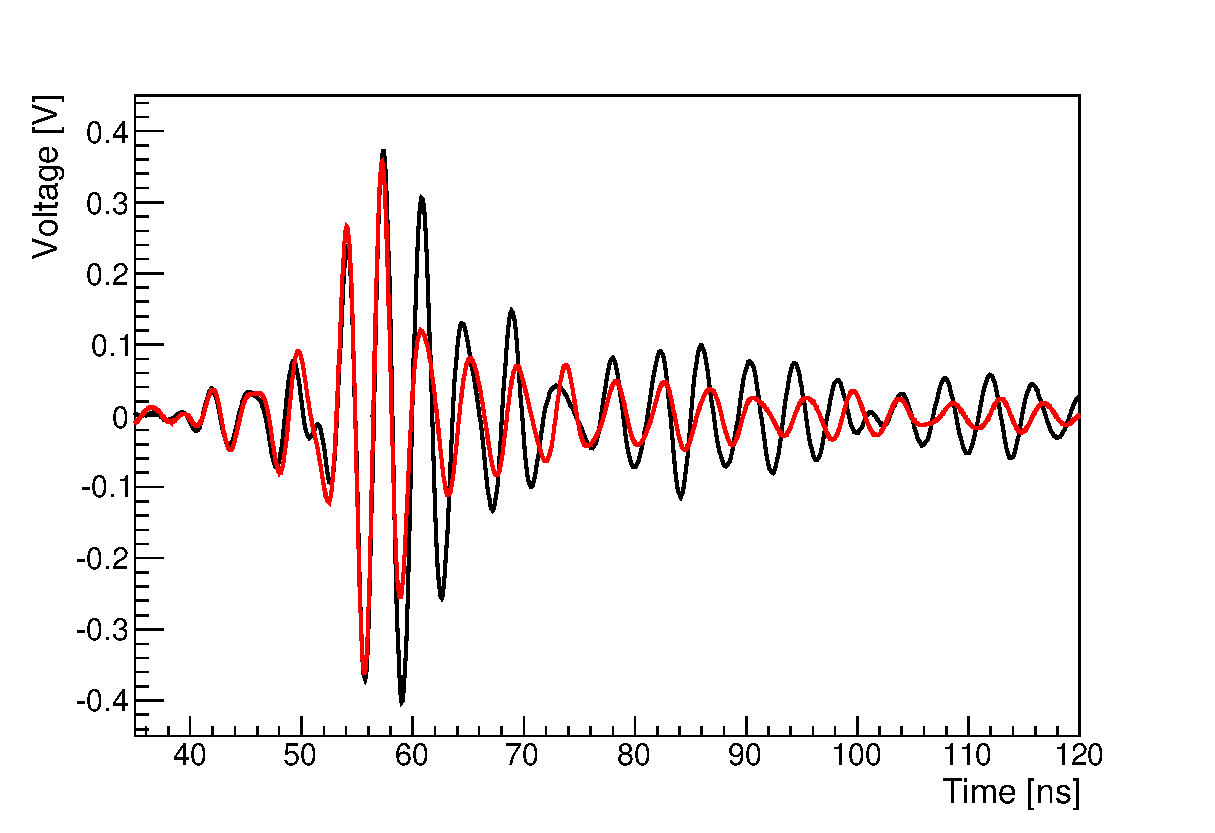
\includegraphics[width=0.47\linewidth]{waveformkeiichi}}
  \caption{Example of a radio waveform recorded with ARACalTA detector during the run with no ice target.}
  \label{fig:waveform}
\end{figure}

\paragraph{Data description}
We collected data without target at 9 different heights ranging from 0 to 7.4m with respect to the point where the beam exits the container allowing us to probe the sudden appearance intensity at angles from 0 to 45 $^{\circ}$. A typical radio waveform is shown in the Figure~\ref{fig:waveform}. The power is extracted from the waveform after . The charge signal is recorded with the wall current monitor which was first calibrated with the Faraday cup on a dedicated calibration run. The radio signal as a function of the charge is fitted with a power law and the exponent is found to be \color{red} [2.?? +- ?? ]\color{black} indicating pure coherence of the signal. Moreover, the polarization of the signal is almost purely vertical. These linear polarization and the quadratic dependence of the signal with the charge are features expected from the sudden appearance signal. \\ The variation of the measured intensity with the angle is shown in the Figure~\ref{fig:angdist}. The sudden appearance signal is simulated using a realistic charge profile as described in ~\ref{sec:simulation}\color{red} [ cite simulation section ]\color{black}. Then the full detector response is simulated. This includes the convolution of the previously obtained electric field  with a simulated antenna response in the time domain. This voltage is in turn multiplied with the gains of the analogical chain (filter, amplifier and cables). The simulated and measured intensities agrees very well.

\begin{figure}[!h]
  \centering
  \hspace*{-3ex}
  	\subfigure{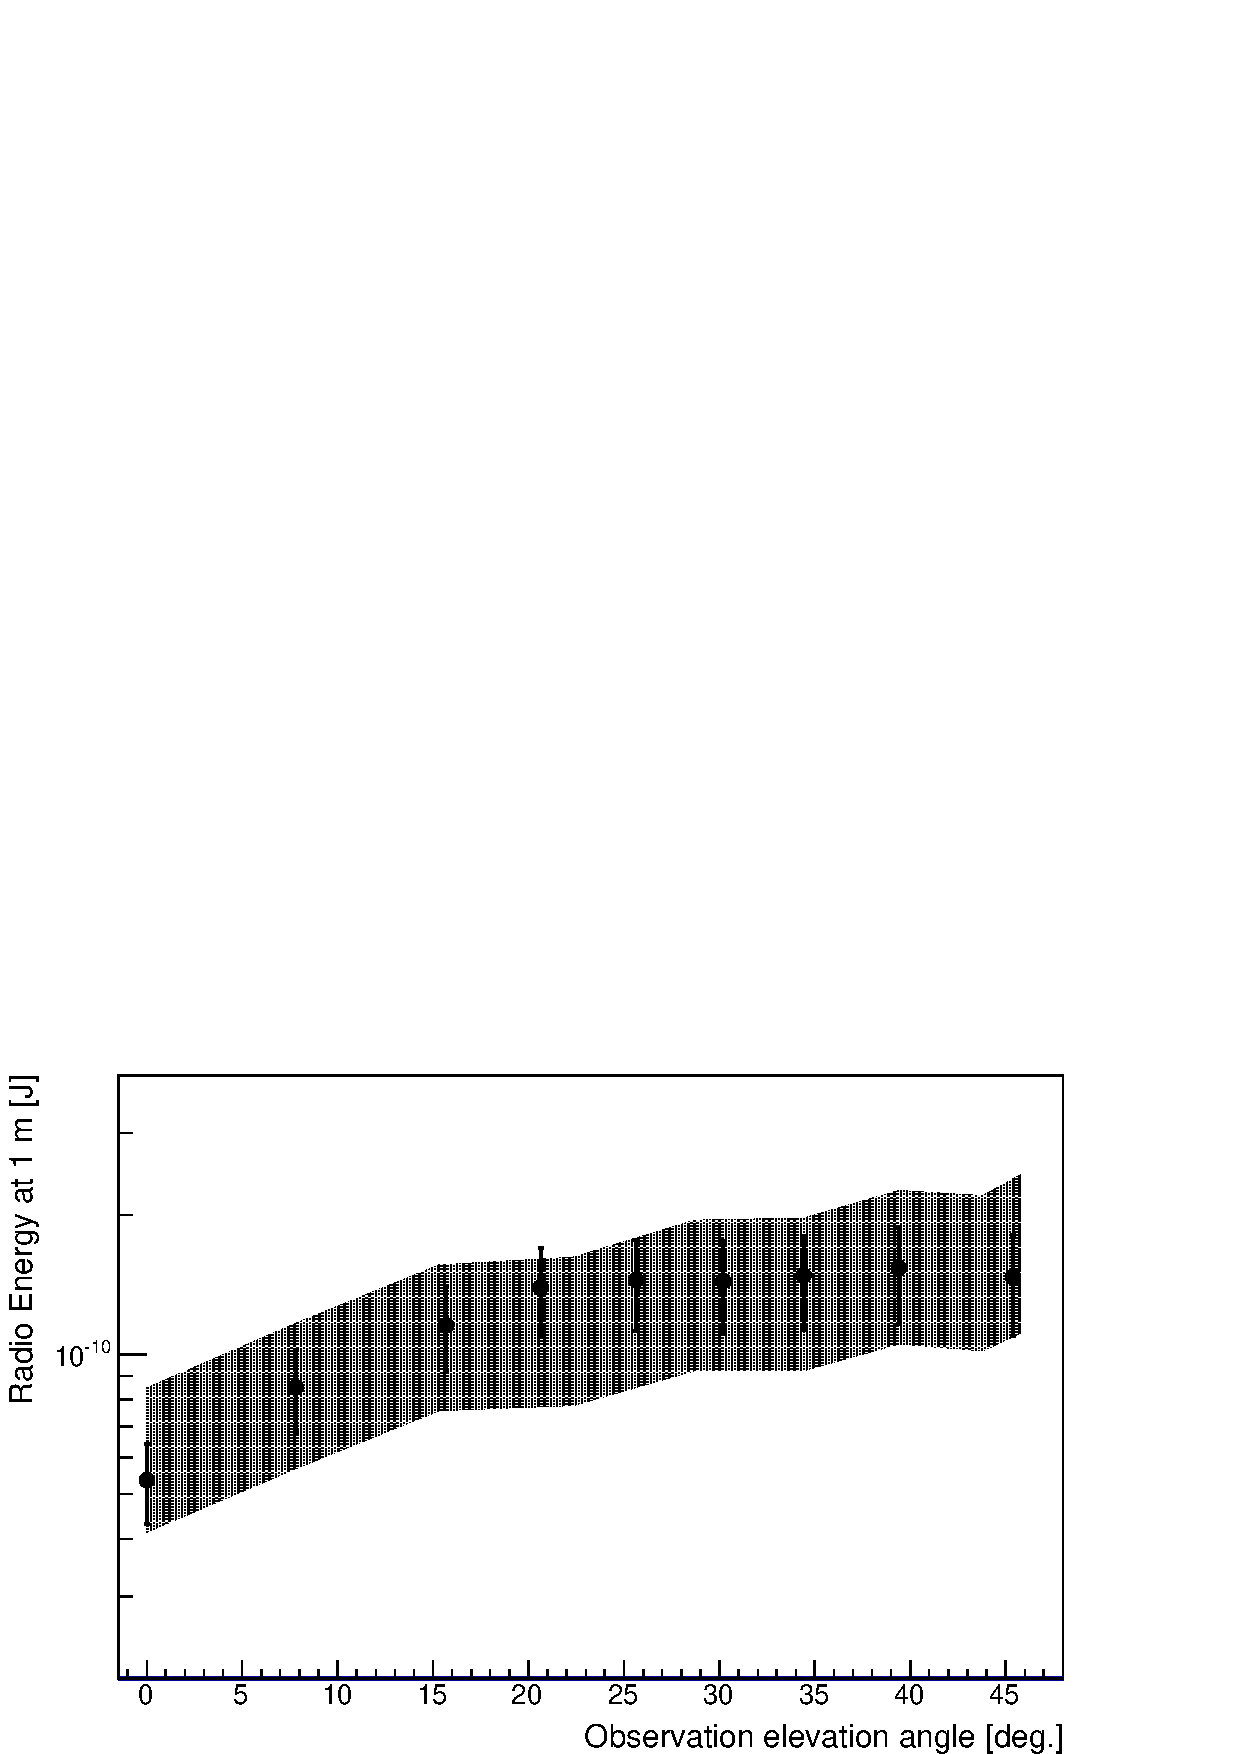
\includegraphics[width=0.52\linewidth]{angulartemporary.jpg}}	        \caption{Angular dependence of the sudden appearance radio energy. The energy is what would be observed at 1 meter. The shaded area is the simulation and the error band accounts for \color{red} ??? \color{black}}
  \label{fig:angdist}
\end{figure}

\end{document}
